\documentclass{article}
\usepackage{hyperref}
\usepackage{tikz}
\usepackage[a4paper]{geometry}
\usepackage{fancyhdr}
\pagestyle{fancy}
\lhead{Gitter}
\rhead{September 2025}
\begin{document}
\section{Das Gitter}
Ein Gitter ist dem \hyperref[Das Doppelspaltexperiment]{Doppelspaltexperiment} sehr ähnlich, nur mit mehr Spalten. Jedes Gitter hat einen Gitterkonstante, dem Spaltabstand, $b$, mit dessen es ein eigenes Interferenzmuster hinterlässt. Es gilt dabei
\[
 k \cdot \Delta = b \cdot \sin{\left(\arctan{\left(\frac{a}{e}\right)}\right)}
\]
 
\subsection{CDs und DVDs} 
\begin{minipage}{\dimexpr\linewidth-4cm}
CDs und DVDs sind eigentlich Gitter. Die Daten, welche auf ihnen gespeichert werden, sind in kleinen Einkerbungen Enkodiert. Wird eine CD nun als Gitter genutzt, welches das Licht eines Lasers reflektiert und beugt, so kann ein einfacher Schirm davorgesetzt werden. Mithilfe von diesem kann nun die obige, bereits bekannte, Formel genutzt werden um die Sitation zu beschreiben. So kann beispielsweise die Gitterkonstante, also der Abstand dieser Einkerbungen, bestimmt werden.
\end{minipage}
\hfill
\begin{minipage}{4cm}
 \center
 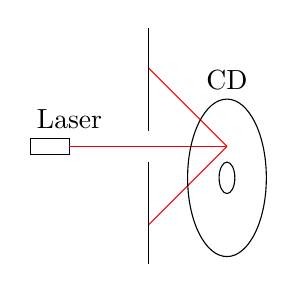
\begin{tikzpicture}
  \draw (-0.5, -0.1) rectangle (0, 0.1) node[above] {Laser};
  \draw[red] (0, 0) -- (2, 0);
  \draw[red] (2, 0) -- (1, -1);
  \draw[red] (2, 0) -- (1, 1);
  \draw (1, 0.2) -- (1, 1.5);
  \draw (1, -0.2) -- (1, -1.5);
  \draw (2,-0.4) ellipse (0.5cm and 1cm);
  \draw (2,-0.4) ellipse (0.1cm and 0.2cm);
  \draw (2, 0.6) node[above] {CD};
 \end{tikzpicture} 
\end{minipage} 
\end{document}